\section{Analisi}
Inizialmente sono state condotte una serie di analisi allo scopo principale di identificare il modello che ha restituito i risultati più promettenti. Successivamente, ci si è dedicati all'indagine delle configurazioni ottimali del momento, al fine di massimizzare l'accuratezza.
\subsection{Scelta del Modello}
Per identificare il modello ottimale, sono stati condotti diversi approfondimenti. Per il primo approfondimento è stata impiegata una rete nota come \textbf{LeNetColor}, successivamente una rete basata su AlexNet, denominata \textbf{MiniAlexNet}, ed infine, dopo aver introdotto sia layer di Dropout che layer di Batch Normalization, abbiamo ottenuto la versione \textbf{MiniAlexNetV2}. 

\begin{figure}[htbp]
\centering
\begin{minipage}[t]{0.33\textwidth}
    \centering
    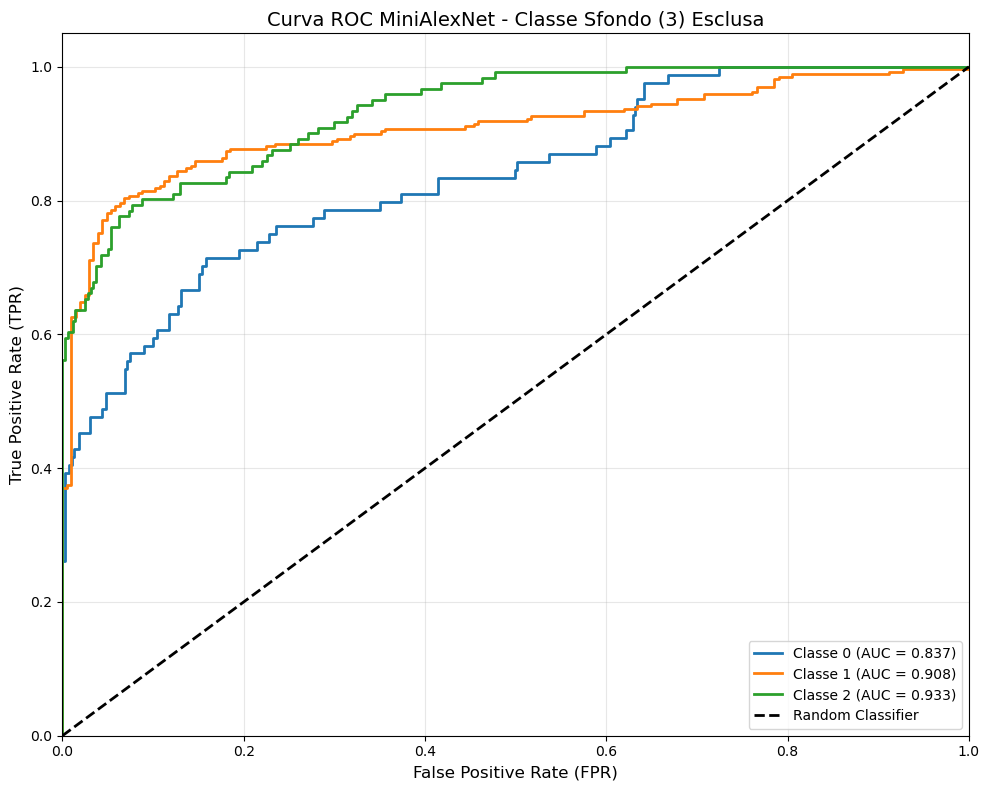
\includegraphics[width=\linewidth]{Analisi/LeNetColor_ROC.png}
\end{minipage}\hfill
\begin{minipage}[t]{0.34\textwidth}
    \centering
    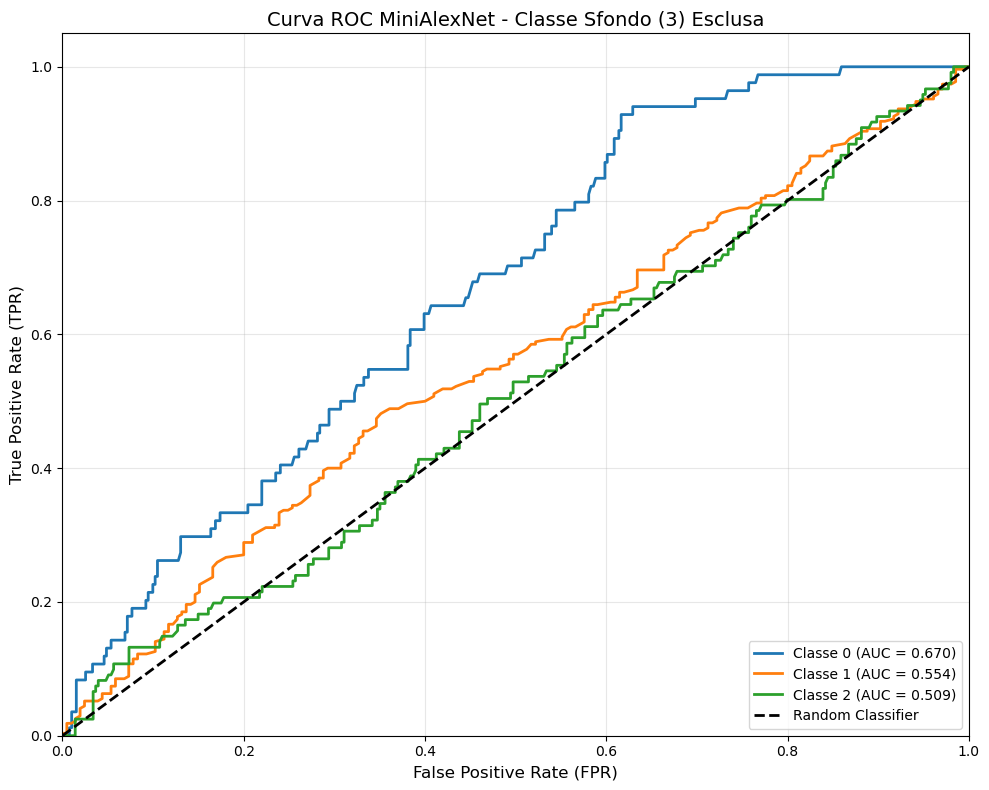
\includegraphics[width=\linewidth]{Analisi/MiniAlexNet_ROC.png}
\end{minipage}\hfill
\begin{minipage}[t]{0.33\textwidth}
    \centering
    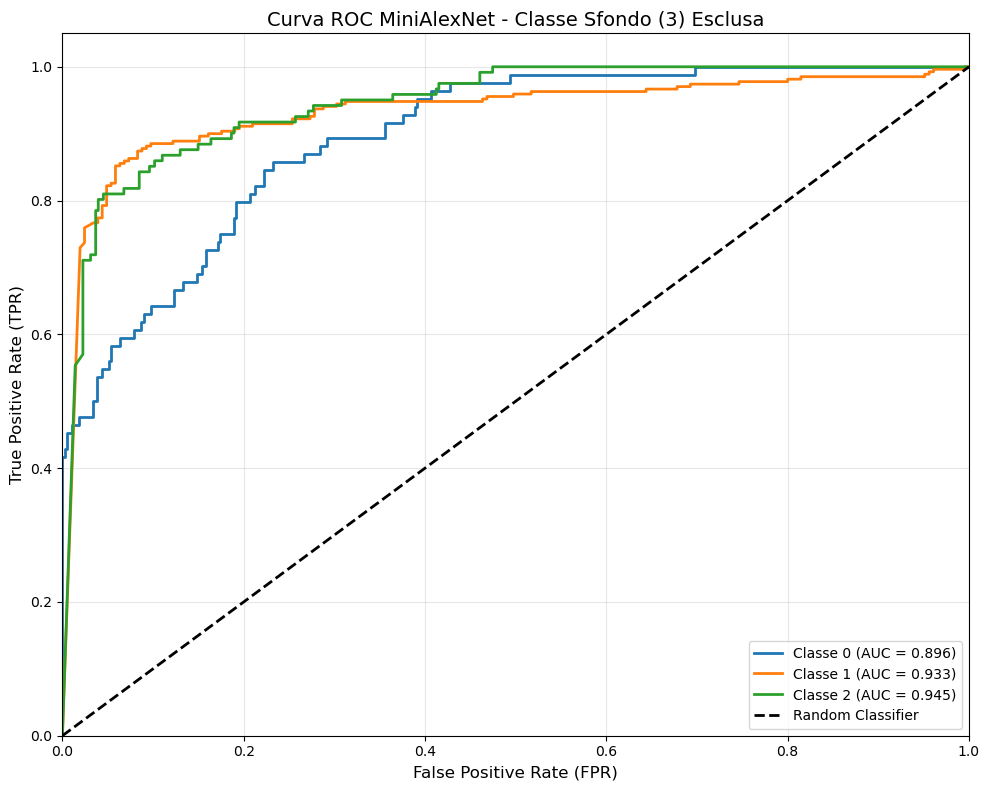
\includegraphics[width=\linewidth]{Analisi/MiniAlexNetV2_ROC.png}
\end{minipage}\hfill

\caption{Confronto tra le ROC curve delle tre reti}
\label{fig:Roc}
\end{figure}

L'esame della Figura  \ref{fig:Roc} evidenzia in modo netto come la rete MiniAlexNetV2 raggiunga un'accuratezza notevolmente superiore rispetto alla MiniAlexNet, che mostra, al contrario, un comportamento oscillante. Sebbene la AlexNet presenti un andamento migliore rispetto alla MiniAlexNet, essa rimane comunque inferiore alla MiniAlexNetV2. Pertanto, dal punto di vista dell'accuratezza, la rete MiniAlexNetV2 emerge come la più efficace.

\begin{figure}[H]
    \centering
    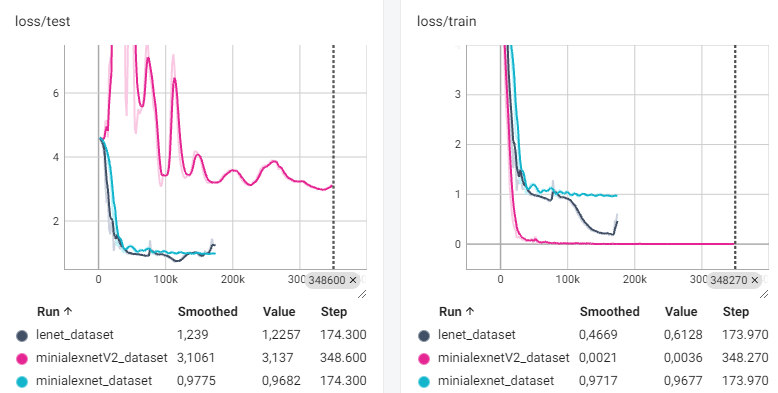
\includegraphics[scale=0.8]{Analisi/ConfrontoLoss.png}
    \caption{Comparazione tra curve loss}
    \label{ConfrontoLoss}
\end{figure}

Dall'analisi della Figura \ref{ConfrontoLoss}, emergono notevoli differenze tra le reti MiniAlexNetV2, MiniAlexNet, e AlexNet, le quali sono state addestrate rispettivamente per 200 epoche durante la fase di training. La rete MiniAlexNetV2 mostra valori di loss inferiori rispetto alle altre due reti.

Tuttavia, durante la fase di test, la curva della MiniAlexNetV2 mostra inizialmente un picco, indicativo di una probabile fase di overfitting nelle prime epoche. Successivamente, la curva si stabilizza su valori di loss più contenuti. Questo comportamento sottolinea la complessità dell'addestramento e la necessità di valutare attentamente le dinamiche della loss durante l'intero processo di addestramento e test. \\
Questi risultati hanno indotto la concentrazione degli sforzi sull'ulteriore sviluppo della rete MiniAlexNetV2. \\
I parametri utilizzati per queste prove sono stati:

\begin{itemize}
  \item Tasso di apprendimento (\textit{Learning Rate}): 0.0001
  \item Momento (\textit{Momentum}): 0.6
\end{itemize}

\subsection{ROC Curve}
Trovati quindi modello e momento, come mostrato prima, è stato reiterato il processo di training, allenando le reti per altre 200 epoche e calcolando la ROC Curve, come mostrato in Figura \ref{fig:Roc}. La curva ROC, che rappresenta la relazione tra il tasso di veri positivi (TPR) e il tasso di falsi positivi (FPR) al variare della soglia di classificazione, è stata utilizzata per valutare le prestazioni del modello in modo più dettagliato.

\begin{figure}[htbp]
\centering
\begin{minipage}[t]{0.33\textwidth}
    \centering
    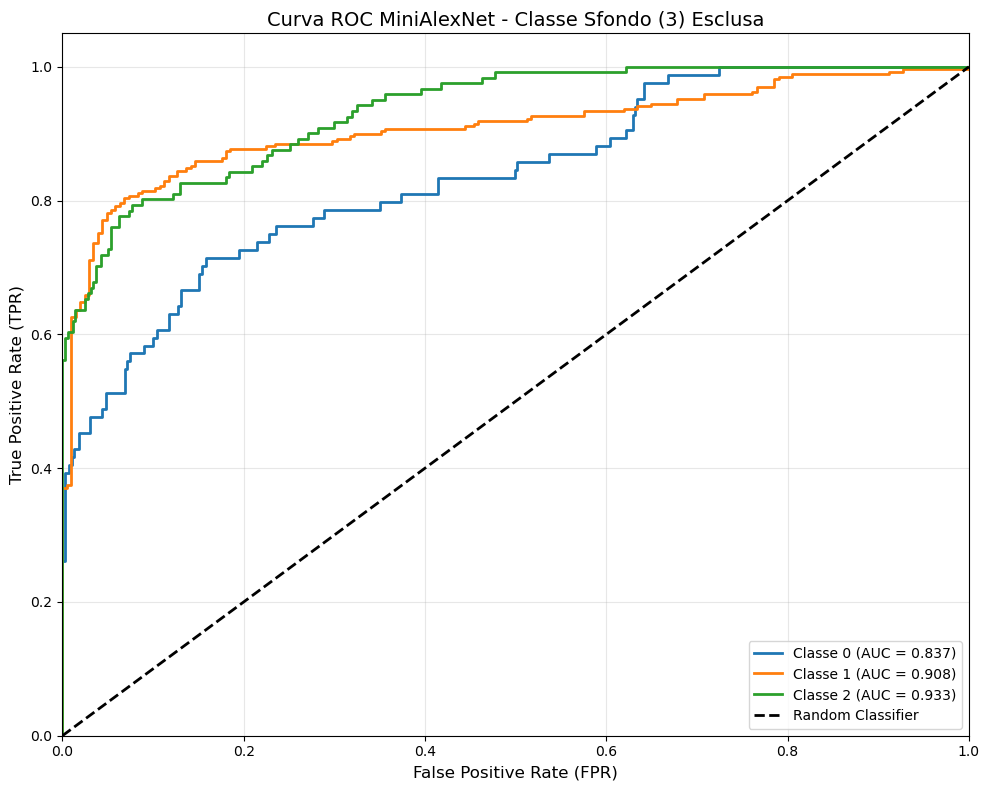
\includegraphics[width=\linewidth]{Analisi/LeNetColor_ROC.png}
\end{minipage}\hfill
\begin{minipage}[t]{0.34\textwidth}
    \centering
    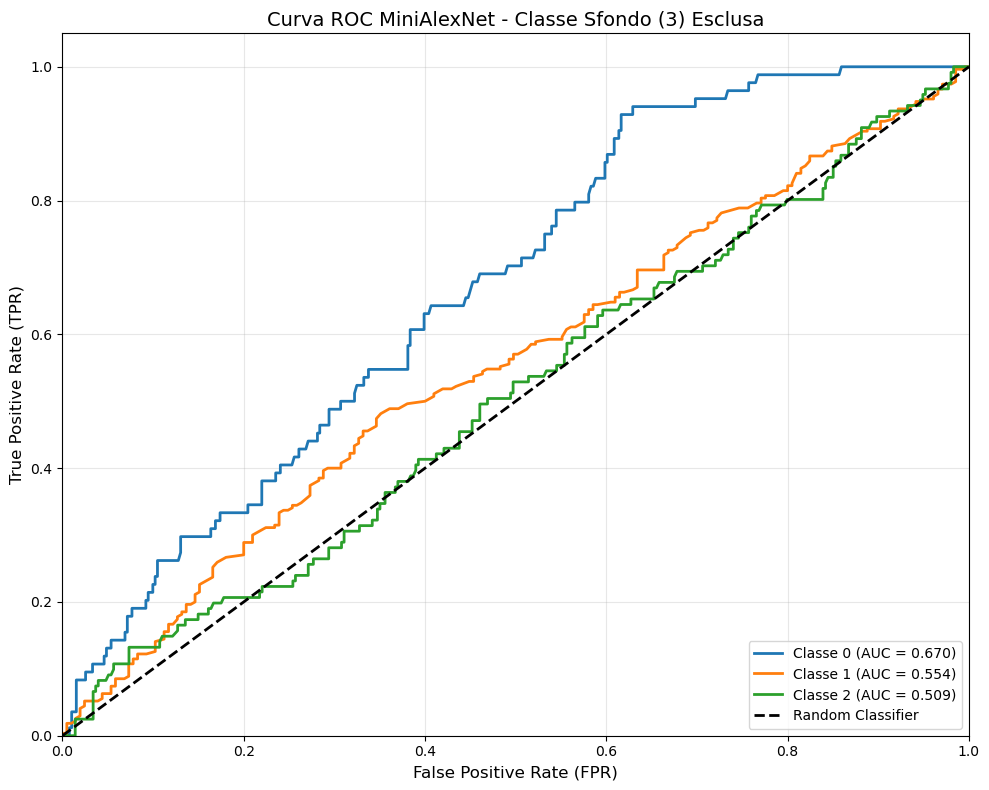
\includegraphics[width=\linewidth]{Analisi/MiniAlexNet_ROC.png}
\end{minipage}\hfill
\begin{minipage}[t]{0.33\textwidth}
    \centering
    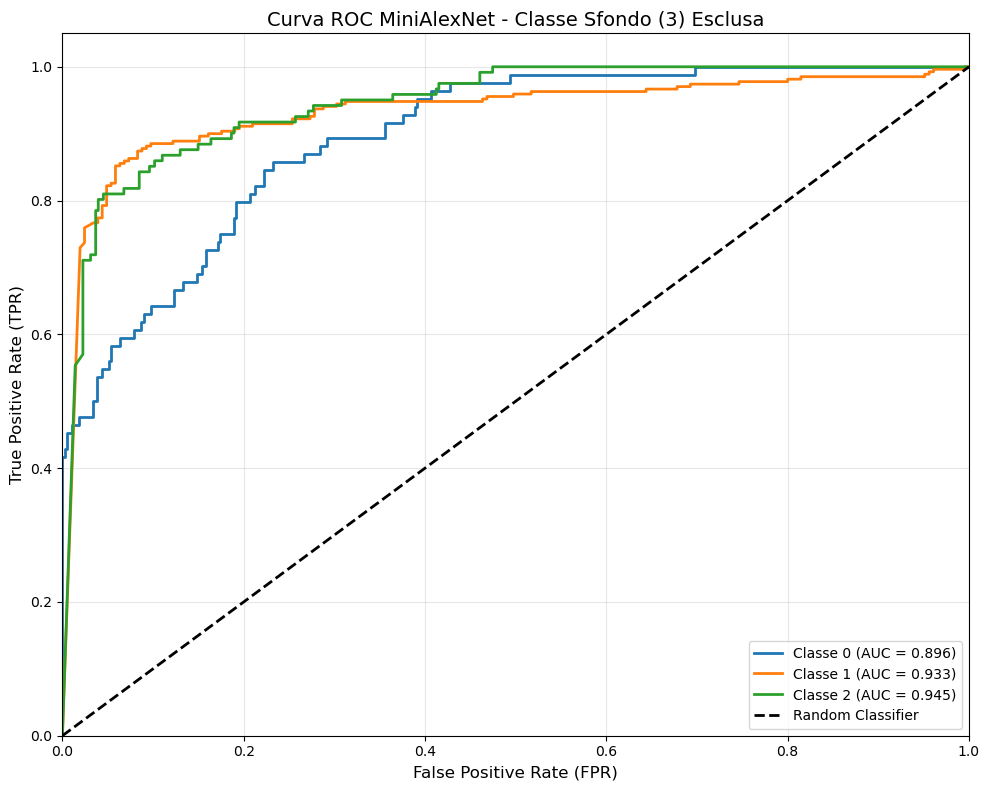
\includegraphics[width=\linewidth]{Analisi/MiniAlexNetV2_ROC.png}
\end{minipage}\hfill

\caption{Confronto tra le ROC curve delle tre reti}
\label{fig:Roc}
\end{figure}

\newpage 

\subsection{Calibrazione del Momento}
Una volta definito il modello, sono stati dedicati sforzi all'ottimizzazione del momento al fine di calibrarlo al meglio. Per valutare l'efficacia di diverse opzioni di momento, ho considerato solo quale tra i valori proposti conducesse a un aumento dell'accuratezza congiuntamente a una convergenza della loss verso valori inferiori.

I dati sull'accuratezza e sulla loss durante l'addestramento del precedente esperimento con MiniAlexNetV2 sono stati conservati. Successivamente, la rete è stata nuovamente addestrata utilizzando un valore di momento pari a 0.7.
I risultati di questo test sono illustrati nella Figura \ref{ConfrontoCurve}. \\ Come evidenziato, il modello presenta un'accuratezza leggermente superiore durante la fase di addestramento e test quando il momento è impostato a 0.6. Le curve di loss convergono a valori leggermente inferiori e seguono un andamento poco più regolare.

Sulla base di tali risultati, si è proceduto mantenendo un valore di momento pari a 0.6.
 
\begin{figure}[H]
    \centering
    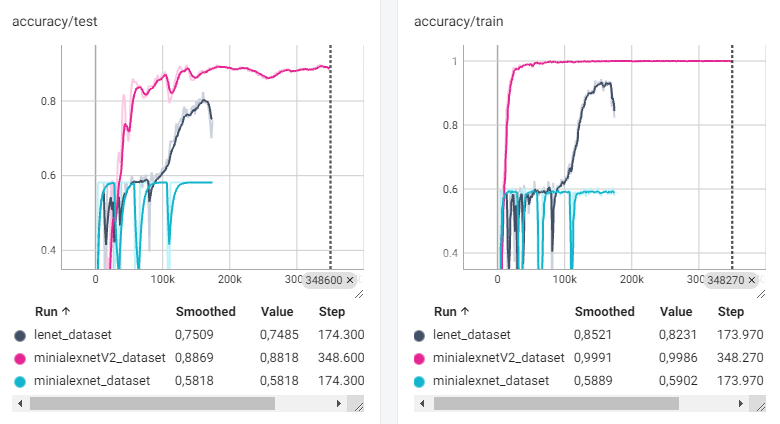
\includegraphics[scale=0.7]{Analisi/ConfrontoAccuracySmooth0.7.png}
    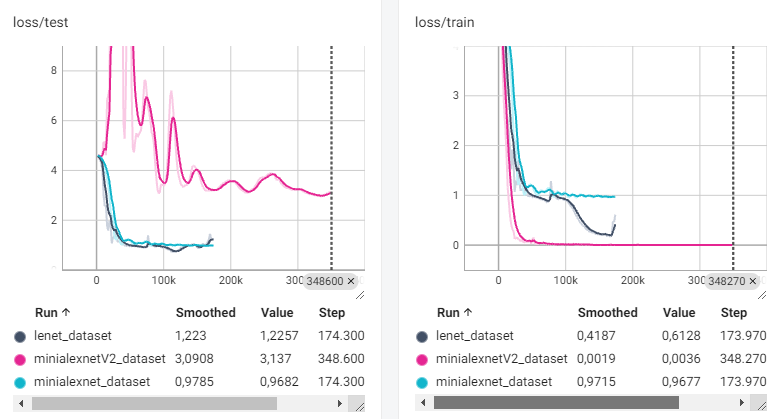
\includegraphics[scale=0.7]{Analisi/ConfrontoLossSmooth0.7.png}
    \caption{Comparazione tra curve accuracy sopra, tra curve loss sotto.}
    \label{ConfrontoCurve}
\end{figure}
\newpage